\documentclass[12pt,a4paper]{report}

\usepackage[utf8]{inputenc}
\usepackage{amsmath}
\usepackage{amsfonts}
\usepackage{amssymb}
\usepackage{hyperref}
\usepackage{graphicx}
\usepackage{titlesec}
\usepackage[francais]{babel}
\usepackage[left=2cm,right=2cm,top=2cm,bottom=2cm]{geometry}

% Personnalisation des chapitres
\titleformat{\chapter}[hang]
{\fontfamily{cmss}\bfseries\huge}{\Roman{chapter} -- }{0cm}{
    \vspace{1ex}
}

% Personnalisation des sections
\titleformat{\section}[hang]
{\bfseries\Large}{\arabic{section} -- }{0cm}{
    \vspace{1ex}
}

\title{PJE\\\#Currentmood}
\author{Quentin Van de Kadsye \and Jérôme Tanghe}
\date{Mardi 15 décembre 2015}

\setlength{\parskip}{\baselineskip}

\begin{document}
\maketitle

\tableofcontents

% -----------------------------------------------------------------------------

\chapter{Le projet}

Il est parfois intéressant pour les entreprises de connaître l'humeur générale
des gens concernant un sujet donné. Twitter étant une plateforme où l'on peut
s'exprimer librement, c'est donc un emplacement de choix pour récolter ce type
d'information. Se pose alors le problème suivant : comment connaître rapidement
l'humeur des personnes sur un sujet donné?

\textbf{\#Currentmood} est un programme tentant de répondre à ce besoin. Écrit
en Java, il permet d'estimer l'humeur d'un ou plusieurs messages publiés sur
Twitter (\textit{tweet}), à l'aide d'une des trois méthodes proposées:

\begin{itemize}
    \item
        \textbf{Mots-clés:} utilise une liste de mots prédéfinis dans des
        fichiers pour déterminer l'humeur du tweet.
    \item
        \textbf{KNN:} évalue l'humeur d'un tweet en fonction de l'humeur de $k$
        autres tweets, en recherchant dans une base de données de tweets dont on
        connaît déjà l'humeur ceux qui contiennent les mêmes mots.
    \item
        \textbf{Classification bayésienne:} évalue la probabilité d'humeur d'un
        tweet en calculant la probabilité que les mots qu'il contient
        appartiennent à cette humeur à partir de la base de données.
\end{itemize}

% TODO insérer capture d'écran

% -----------------------------------------------------------------------------

\chapter{API Twitter et gestion des tweets}

\section{La classe \texttt{CMTwitter}}

Afin de communiquer avec l'API de Twitter, nous avons utilisé la librairie
\textbf{Twitter4J}\footnote{\href{http://twitter4j.org}{twitter4j.org}} qui
propose les fonctionnalités dont nous avons besoin pour mener à bien le projet.
Pour faciliter son implémentation, nous avons également créé une classe,
\texttt{CMTwitter}, s'interfaçant entre notre application et Twitter4J, comme le
montre la figure \ref{uml_cmtwitter}.

\begin{figure}[h]
    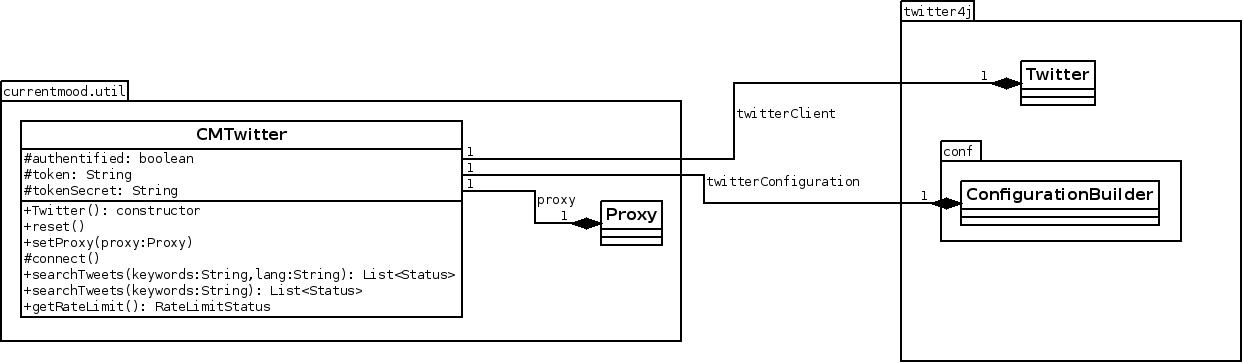
\includegraphics[width=1\textwidth]{img/uml_cmtwitter.png}
    \caption{Diagramme de classe montrant comment nous interfaçons Twitter4J}
    \label{uml_cmtwitter}
\end{figure}

Cela nous permet d'utiliser l'API de Twitter à l'aide de trois méthodes
principales seulement au lieu d'une dizaine:

\begin{itemize}
    \item
        \texttt{setProxy()} afin de donner les paramètres proxy à Twitter4J;
    \item
        \texttt{connect()} afin d'établir la connexion avec l'API de Twitter;
    \item
        \texttt{searchTweets()} afin d'utiliser la fonction de recherche de
        l'API de Twitter.
\end{itemize}

La méthode \texttt{reset()}, quant à elle, est utilisée par les méthodes
précédentes afin de permettre d'effectuer plusieurs requêtes. En effet, nous
avons pu remarquer que l'objet \texttt{ConfigurationBuilder} périme après chaque
requête, nous obligeant à le recréer avant d'effectuer une nouvelle requête.

L'utilisation de cette classe s'effectue en trois étapes principales.

Tout d'abord, on configure si nécessaire les paramètres proxy à l'aide de la
méthode \texttt{setProxy()}. Cette dernière donne lesdits paramètres à l'objet
\texttt{ConfigurationBuilder}.

Ensuite, on appelle la méthode \texttt{connect()} qui utilise l'objet
\texttt{ConfigurationBuilder} pour obtenir une instance de \texttt{Twitter}.

C'est cette instance qui est ensuite utilisée par \texttt{searchTweets()} qui
instancie un objet de Twitter4J permettant d'obtenir des tweets correspondant
à la recherche. Cette méthode retourne une liste d'objets \texttt{Status}
provenant de la librairie Twitter4J.

\section{La classe \texttt{Tweet}}

Nous nous sommes rapidement rendus compte que Twitter4J ne proposait aucune
classe implémentant l'interface \texttt{Status} que nous devons manipuler. De
plus, les objets que nous en obtenons contient de nombreuses informations qui ne
nous sont pas utiles, tandis que d'autres nous étaient nécessaires mais
n'y étaient pas présents.

Nous avons donc créé une classe indépendante de Twitter4J, \texttt{Tweet}, qui
réponde à ce besoin. Elle est utilisée dans toute l'application afin de contenir
chaque tweet.

\begin{figure}[h]
    \centering
    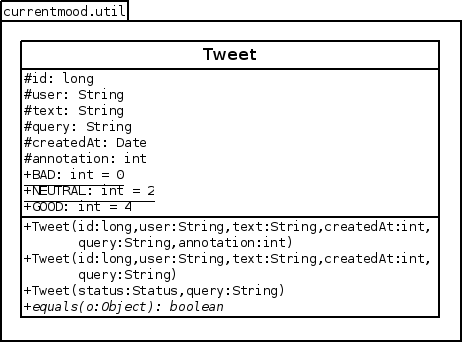
\includegraphics[width=7cm]{img/uml_tweet.png}
    \caption{La classe \texttt{Tweet}}
    \label{uml_tweet}
\end{figure}

Cette classe est surtout composée d'accesseurs permettant d'accéder à chaque
propriété du tweet. Ses deux premiers constructeurs permettent de créer un objet
à partir de données déjà connues (typiquement lors de l'ouverture d'un fichier
CSV), tandis que le troisième permet d'obtenir un objet \texttt{Tweet} à partir
d'un objet \texttt{Status} généré par Twitter4J.

Nous avons également surchargé la méthode \texttt{equals()} de la super-classe
\texttt{Object} afin de permettre la comparaison de l'objet courant avec un
autre objet \texttt{Tweet}. Cela nous sera nécessaire pour certaines actions par
la suite.

\section{Le fichier CSV}

Pour gérer la base de données, il a été décidé de sauvegarder les messages
annotés dans un fichier CSV\footnote{\textit{Comma-separated values}}. Ce type
de fichier a pour principal avantage d'être relativement léger et facile à lire
par programmation.

Les données à sauvegarder étant globalement celles contenues dans les objets
\texttt{Tweet}, l'ordre de sauvegarde sera donc le suivant:

\begin{enumerate}
    \item
        Le numéro d'identification du tweet
    \item
        Le nom de l'auteur du tweet
    \item
        Le contenu du tweet
    \item
        La date et l'heure du tweet
    \item
        La recherche qui a permi de trouver le tweet
    \item
        L'annotation du tweet
\end{enumerate}

\end{document}
